\documentclass{article}
\usepackage[utf8]{inputenc}
\usepackage{amsmath}
\usepackage{amssymb}
\usepackage{graphicx}
\graphicspath{{Images/}}



\setlength{\oddsidemargin}{0in}
\setlength{\textwidth}{6.5in}
\setlength{\topmargin}{-.55in}
\setlength{\textheight}{9in}
\pagestyle{empty}



\title{Problem Set 8 (Astrophysics)}
\author{Michael Nameika}
\date{April 2022}

\begin{document}

\maketitle

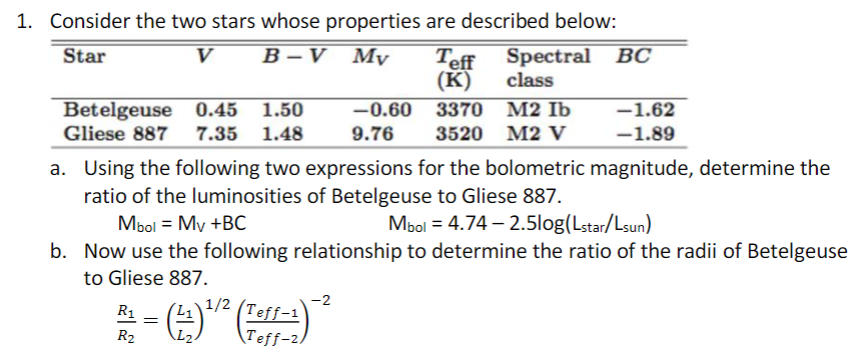
\includegraphics[scale = 0.8]{probset8prob1.PNG}

a) Using the first equation for the bolometric magnitude to calculate the bolometric magnitude for Betelgeuse and Gliese 887, we find
\[M_{Bol,B} = -0.60 - 1.62 = -2.22\]
\[M_{Bol,G} = 9.76 - 1.89 = 7.87\]
And now, using the second equation for bolometric magnitude, we can solve for the luminosity of Betelgeuse and Gliese 887. Notice that
\[L_{Star} = L_{Sun}(10^{\frac{4.74 - M_{Bol}}{2.5}})\]
and so 
\[L_{Betelgeuse} = L_{Sun}(10^{\frac{4.74 + 2.22}{2.5}})\]
\[ = L_{Sun}(10^{\frac{6.96}{2.5}})\]
and
\[L_{Gliese \:887} = L_{Sun}(10^{\frac{4.74 - 7.87}{2.5}})\]
\[ = L_{Sun}(10^{\frac{-3.13}{2.5}})\]
And so the ratio between the luminosities of Betelgeuse and Gliese 887 is given by
\[\frac{L_{Betelgeuse}}{L_{Gliese \:887}} = \frac{L_{Sun}(10^{6.96/2.5})}{L_{Sun}(10^{-3.13/2.5})}\]
\[ = 10^{\frac{10.09}{2.5}}\]
\[\approx 10860\]
So Betelgeuse is approximately 10,860 times more luminous than Gliese 887.

b) Using the values given in the table for the temperature of Betelgeuse and Gliese 887, and the values for the ratio of their luminosities, we find that
\[\frac{R_{Betelgeuse}}{R_{Gliese \:887}} = \left(\frac{L_{Betelgeuse}}{L_{Gliese \:887}}\right)^{1/2}\left(\frac{3370}{3520}\right)^{-2}\]
\[\approx (10860)^{1/2}\left(\frac{3370}{3520}\right)^{-2}\]
\[\approx 113.7\]
So Betelgeuse is approximately 113.7 times larger than Gliese 887 in radius.
\newline

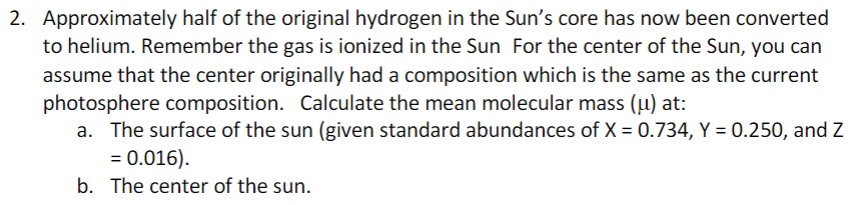
\includegraphics[scale = 0.8]{probset8prob2.PNG}
\newline

a) 
\[\mu = (2X + \frac{3Y}{4} + \frac{Z}{2})^{-1}\]
\[ = (1.468 + \frac{0.750}{4} + \frac{Z}{2})^{-1}\]
\[\approx 0.601\]

b) Since the composition is assumed to be the same in the center of the sun, we will find the same result, $\mu \approx 0.601$.

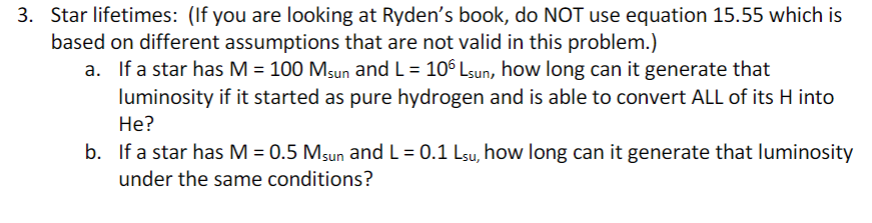
\includegraphics[scale = 0.8]{probset8prob3.PNG}
\newline

Recall that the lifetime of the sun is estimated to be approximately 10 billion years and that the lifetime can be approximated using the following formula:
\[\tau = \frac{E}{L}\]
where $E$ is the available energy of the star and $L$ is the luminosity. Also recall that $E \propto M$.

a) Given that $M = 100 \: M_{Sun}$ and $L = 10^6 \: L_{Sun}$, we have that 
\[\tau = \frac{100 E_{Sun}}{10^6 L_{Sun}}\]
\[ = 10^{-4} (10 \times 10^9 \:\text{years})\]
\[ = 10^6 \: \text{years}\]

b) Given that $M = 0.5 \:M_{Sun}$ and $L = 0.1 \:L_{Sun}$, we have that
\[\tau = \frac{0.5 \:E_{Sun}}{0.1 \:L_{Sun}}\]
\[ = 5 (10 \times 10^9 \: years)\]
\[ = 50 \: \text{billion years} \]



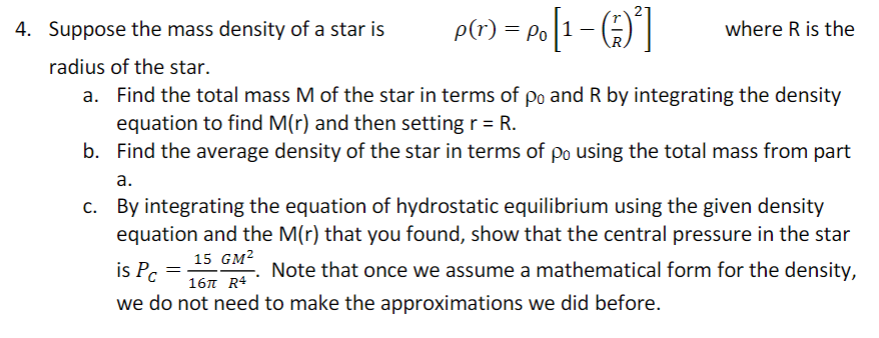
\includegraphics[scale = 0.8]{probset8prob4.PNG}
\newline

a) Notice that the mass of the star as a function of $r$ is given by
\[M(r) = \int \int \int_{\Omega} \rho(r) dV\]
which becomes
\[M(r) = \int_0^{2\pi} \int_0^{\pi} \int_0^r \rho_0\left[1 - \left(\frac{r}{R}\right)^2\right]r^2 \sin{(\phi)} drd\phi d\theta\]
Solving we find
\[M(r) = 4\pi \rho_0\left[\frac{r^3}{3} - \frac{r^5}{5R^2}\right]\]
and plugging in $r = R$ to find the total mass:
\[M = \frac{8\pi \rho_0}{15}R^3\]

b) To find the average density, we must divide the total mass by the volume of the star (assuming spherical volume):
\[\frac{M}{V} = \left(\frac{8\pi \rho_0}{15}R^3\right)/\left(\frac{4}{3}\pi R^3\right)\]
and we find that
\[\rho_{avg} = \frac{2}{5}\rho_0\]

c) Recal the equation for hydrostatic equilibrium is given by
\[\frac{dP}{dr} = -\frac{GM(r)\rho(r)}{r^2}\]
Integrating this equation from $r = 0$ to $r = R$, we find that
\[P(R) - P(0) = -G\int_0^R \frac{M(r)\rho(r)}{r^2}dr\]
which becomes
\[P_C = G \int_0^R \frac{M(r)\rho(r)}{r^2}dr\]
and plugging in the expressions we found for $M(r)$ and $\rho(r)$, we find
\[P_C = G\int_0^R 4\pi \rho_0^2\left[\frac{r^3}{3} - \frac{r^3}{5R^2}\right]\]
\[ = 4\pi G\rho_0^2 \int_0^R\left[\frac{r}{3} - \frac{8r^3}{15R^2} + \frac{r^5}{5R^4}\right]dr\]
\[ = 4\pi G\rho_0^2\left(\frac{R^2}{6} - \frac{2R^2}{15} + \frac{R^2}{30}\right)\]
\[ = 4\pi G \rho_0^2\left(\frac{R^2}{15}\right)\]
And notice from our work above that 
\[\rho_0 = \frac{15M}{8\pi R^3}\]
and so
\[P_C = \frac{4\pi}{15}G\left(\frac{15^2M^2}{64 \pi^2R^6}\right)R^2\]
\[ = \frac{15 M^2G}{16 \pi R^4}\]
Which is the result we wished to show.


\end{document}
